\documentclass{article}
\usepackage[utf8]{inputenc}

\title{Predicting Student Demand}
\author{Edderic Ugaddan}
\date{September 2016}

\usepackage{natbib}
\usepackage{graphicx}
\usepackage{amsmath, amsthm, amssymb}
\usepackage{url}
\usepackage{bbding}
\usepackage{array}

\DeclareMathOperator*{\argmin}{argmin}
\DeclareMathOperator*{\argmax}{argmax}
\newcolumntype{P}[1]{>{\centering\arraybackslash}p{#1}}

\begin{document}

\maketitle


\section{Definition}

\subsection{Project Overview}
Lingo Live provides customized communication lessons for tech professionals.
We specialize in providing engineers in multinational tech companies, many of
whom are non-native speakers, a language/communication teacher who knows
exactly what they need, anytime and anywhere. Breaking down language and
communication barriers helps them become more effective communicators, and
therefore, improves their career potential.

It is important for us to make sure that our supply of teachers is able to meet
student demand. As part of the tech team at Lingo Live, one of my
responsibilities is to provide accurate forecasts on our capacity to handle
future students -- do we have enough capacity to handle an influx of new
students? If so, how much more can we handle? If not, how many more teachers do
we need to hire, and what times should they be teaching? Underestimating and
overestimating capacity has serious consequences; hiring not enough teachers
means that some or many students won't be able to get lessons at times that
they want. On the other hand, if we hire too many teachers, many of them might
not get enough lessons, and might have to look at other sources of income to
supplement the income they get from Lingo Live. Thus, getting accurate
forecasts of teacher capacity would help our students and teachers stay happy.

The process of analyzing our capacity involves two main stages. First,
predicting student demand given indirect information, such as timezone of these
students, which company they are working for, a ballpark number of students
that are coming in, and the supposed lesson frequency that people will be
taking.  We would generate a bunch of possible schedules that these new
students might have, based on current student data. Finally, once we have these
predicted schedules, we then compare them with current teacher availability to
see how much we could handle. My focus for this project is only the first stage
-- given timezone and company data, could we generate schedules that are
representative of the new students?

Data used in this project is from Lingo Live's production database, anonymized
to protect students' and companies' privacy.

\subsection{Problem Statement}

\subsubsection{Main Idea}

The end goal is to be able to create a model that generates potential students'
schedules very well, so that Lingo Live could find the balance between
under-hiring and over-hiring teachers. The challenge I would like to address is
creating a model that predicts student demand (i.e. when lesson requests are
generally likely to occur in the context of the week) for new students -- see
Table \ref{tab:student_schedule_example} for an example of a student schedule.

\begin{table}[]
  \centering
  \caption{Example of a Student Weekly Schedule}
  \label{my-label}
  \begin{tabular}{|P{1cm}|P{1cm}|P{1cm}|P{1cm}|P{1cm}|P{1cm}|P{1cm}|P{1cm}|}
    \hline
                  & \textbf{Mon} & \textbf{Tue} & \textbf{Wed} & \textbf{Thu} & \textbf{Fri} & \textbf{Sat} & \textbf{Sun} \\
    \textbf{0:00} &  & \Checkmark & & & & & \Checkmark \\
    \textbf{0:15} &  & & \Checkmark & & & &\\
    \textbf{0:30} &  & & & & & &\\
    \textbf{.}    &. &. &. &. &. &. &.\\
    \textbf{.}    &. &. &. &. &. &. &.\\
    \textbf{.}    &. &. &. &. &. &. &.\\
    \textbf{23:30} &  & & & & & &\\
    \textbf{23:45} &  & & & & & &\\
    \hline
  \end{tabular}\label{tab:student_schedule_example}
\end{table}

The strategy to build this model is as follows.  First, I will perform
exploratory data analysis (EDA) to figure out the general trend of user
schedules, using K-Means clustering. K-Means would group like-schedules
together, and would give us "centroids," which are essentially the average
"ideal" member of the clusters. Second, I would make use of the new-found
knowledge to create a model that best predicts when people are going to take
lessons. For benchmarking purposes, I would create two other models. First, I
would create a model that assumes that schedules are distributed equally
(EQ-DIST, Table \ref{tab:eq_dist}).  Second, I would then create a model
that assumes schedules are equally distributed in the range of hours when most
people are active (ACT, Table \ref{tab:act}). Finally, I would compare the performance of these
models across time -- given access to 'previous' months, could these models
predict the 'current' month?

\begin{table}[]
  \centering
  \caption{EQ-Dist Model: Assumes lesson requests (naively) start randomly anytime}
  \label{tab:eq_dist}
  \begin{tabular}{|P{1cm}|P{1cm}|P{1cm}|P{1cm}|P{1cm}|P{1cm}|P{1cm}|P{1cm}|}
    \hline
                  & \textbf{Mon} & \textbf{Tue} & \textbf{Wed} & \textbf{Thu} & \textbf{Fri} & \textbf{Sat} & \textbf{Sun} \\
    \textbf{0:00} & \Checkmark &\Checkmark &\Checkmark &\Checkmark &\Checkmark &\Checkmark &\Checkmark \\
    \textbf{0:15} & \Checkmark &\Checkmark &\Checkmark &\Checkmark &\Checkmark &\Checkmark &\Checkmark \\
    \textbf{0:30} & \Checkmark &\Checkmark &\Checkmark &\Checkmark &\Checkmark &\Checkmark &\Checkmark \\
    \textbf{.}    & \Checkmark &\Checkmark &\Checkmark &\Checkmark &\Checkmark &\Checkmark &\Checkmark \\
    \textbf{.}    & \Checkmark &\Checkmark &\Checkmark &\Checkmark &\Checkmark &\Checkmark &\Checkmark \\
    \textbf{.}    & \Checkmark &\Checkmark &\Checkmark &\Checkmark &\Checkmark &\Checkmark &\Checkmark \\
    \textbf{23:30} & \Checkmark &\Checkmark &\Checkmark &\Checkmark &\Checkmark &\Checkmark &\Checkmark \\
    \textbf{23:45} & \Checkmark &\Checkmark &\Checkmark &\Checkmark &\Checkmark &\Checkmark &\Checkmark \\
    \hline
  \end{tabular}
\end{table}

\begin{table}[]
  \centering
  \caption{ACT Model: Assumes lesson requests only start when people are generally awake}
  \label{tab:act}
  \begin{tabular}{|P{1cm}|P{1cm}|P{1cm}|P{1cm}|P{1cm}|P{1cm}|P{1cm}|P{1cm}|}
    \hline
                  & \textbf{Mon} & \textbf{Tue} & \textbf{Wed} & \textbf{Thu} & \textbf{Fri} & \textbf{Sat} & \textbf{Sun} \\
    \textbf{0:00}    &. &. &. &. &. &. &.\\
    \textbf{0:15}    &. &. &. &. &. &. &.\\
    \textbf{.}    &. &. &. &. &. &. &.\\
    \textbf{.}    &. &. &. &. &. &. &.\\
    \textbf{.}    &. &. &. &. &. &. &.\\
    \textbf{7:45}    &. &. &. &. &. &. &.\\
    \textbf{8:00} & \Checkmark &\Checkmark &\Checkmark &\Checkmark &\Checkmark &\Checkmark &\Checkmark \\
    \textbf{8:15} & \Checkmark &\Checkmark &\Checkmark &\Checkmark &\Checkmark &\Checkmark &\Checkmark \\
    \textbf{.}    & \Checkmark &\Checkmark &\Checkmark &\Checkmark &\Checkmark &\Checkmark &\Checkmark \\
    \textbf{.}    & \Checkmark &\Checkmark &\Checkmark &\Checkmark &\Checkmark &\Checkmark &\Checkmark \\
    \textbf{.}    & \Checkmark &\Checkmark &\Checkmark &\Checkmark &\Checkmark &\Checkmark &\Checkmark \\
    \textbf{19:30} & \Checkmark &\Checkmark &\Checkmark &\Checkmark &\Checkmark &\Checkmark &\Checkmark \\
    \textbf{19:45} & \Checkmark &\Checkmark &\Checkmark &\Checkmark &\Checkmark &\Checkmark &\Checkmark \\
    \textbf{20:00} &. &. &. &. &. &. &.\\
    \textbf{.}    &. &. &. &. &. &. &.\\
    \textbf{.}    &. &. &. &. &. &. &.\\
    \textbf{.}    &. &. &. &. &. &. &.\\
    \textbf{23:30} &. &. &. &. &. &. &.\\
    \textbf{23:45} &. &. &. &. &. &. &.\\
    \hline
  \end{tabular}
\end{table}


\subsubsection{Taming Complexity}

One problem is that the space of possibilities of what we are essentially
trying to predict (i.e. when a student will generally take lessons) is huge,
relative to the feature space (of timezones and lesson frequency). This hurts
our ability to predict when a specific student will precisely take lessons. The
specifics of why this is are explained below.

First, I will establish that the number of possible schedules could be quite
huge. For example, a schedule consists of lesson requests in the context of a
week. A lesson request has two dimensions: day of the week and start time.
There are $7$ days of the week.  Day of the week ranges from $0-6$ ($0$ for
Monday, $1$ for Tuesday, ..., $6$ for Sunday).  Start time is in $15$-minute
increments -- thus, there are $24 \times 4 = 96$ possible start times.
Therefore, a lesson in the context of a schedule could be represented as one of
$7 \times 96 = 672$ possible values.  Thus, a $3$-lesson schedule could be one
of potentially $672 \times 671 \times 670 = 303,464,448$ permutations.

Contrast this with the relatively small hyperspace of predictors -- timezone
and lesson frequency. There are $24$ timezones and $7$ schedule types (e.g.
once a week, twice a week, three times a week, etc.) Thus there are only $24
\times 5 = 120$ combinations of features, which is several orders of magnitude
smaller than the space of schedules we are trying to predict.  Theoretically
speaking, translating from low fidelity (predictors) to very high fidelity
(schedules) could be very difficult. As an analogy, imagine transforming a
pixelated low-resolution picture into a non-pixelated, high-resolution one --
practically impossible to do, since we're trying to add information that we
just don't have (Figure \ref{fig:mona}).

\begin{figure}[h!]
\centering
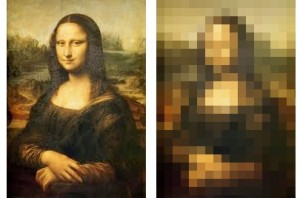
\includegraphics[scale=0.75]{img/pixelmona.jpg}
\caption{Clear vs. Pixelated Mona Lisa -- easy to transform from clear to pixelated, but not the other way around}
\label{fig:mona}
\end{figure}

To simplify the problem of trying to figure out whether one model is better
than another, we would bin the weekly schedule into smaller buckets: 0-4, 4-8,
8-12, 12-16, 16-20, 20-0 UTC. Mapping $120$ combinations of features
into only $6$ buckets becomes a much easier prediction problem.

\subsection{Metrics}

The error metric $e_b$ for bucket $b$ that we are trying to minimize is as follows:

\begin{equation}
  e_b = (y_{b} - \hat{y}_{b})^2
\end{equation}

where $y$ is actual and $\hat{y}$ is predicted.  More specifically, $y_{b}$
is the actual number of lessons that belong to bucket $b$, $\hat{y}_{b}$ is
the predicted number of lessons that belong to bucket $b$.

The total error, considering each bucket, then is just the sum of the errors
for each bucket.

\begin{align}
  Total Error &= \sum_{b=0}^{z}{e_b} \\
              &= \sum_{b=0}^{z}{(y_{b} - \hat{y}_{b})^2}
\end{align}

where $z$ is the total number of buckets.

We would like to be able to compare how much a prediction in one month compares
against other months. The number of lessons from new students per month might
vary considerably, as a function of the number of new students signing up, and
the lesson frequency. Thus, for a certain month $m$, and model $a$, we could
average out the total error by dividing by the number of lessons $n_m$, and get
Mean Squared Error (MSE):

\begin{align}
  MSE(m,a) &= \frac{1}{n_m}\sum_{b=0}^{z}{(y_{(b,m)} - \hat{y}_{(b,m,a)})^2}\\
\end{align}

We would then measure how the models perform over time. We would split our data
into months, and at any point in time, we would use the previous months to
predict the "next" month (i.e. time series cross validation)\cite{tscv}. We would pick the
model $g$ that best minimizes MSE on unseen test data over $o$ months:

\begin{align}
  g &= \argmin_{a}{\frac{ \sum_{m=0}^{o}{MSE(m,a)} }{o}}\\
    &= \argmin_{a}{\frac{ \sum_{m=0}^{o}{ \frac{1}{n_m}\sum_{b=0}^{z}{(y_{(b,m)} - \hat{y}_{(b,m,a)})^2} } }{o}}\\
\end{align}

\section{Analysis}

\subsection{Data Exploration}

\begin{figure}[h!]
\centering
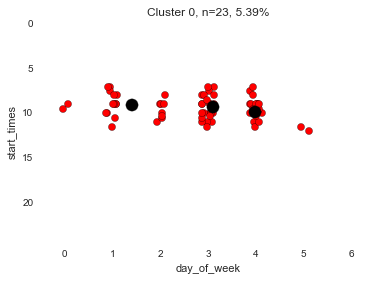
\includegraphics[scale=0.75]{img/2x_cluster_0_out_of_19.png}
\caption{The Universe}
\label{fig:univerise}
\end{figure}

\subsection{Conclusion}
lol

\bibliographystyle{plain}
\bibliography{references}
\end{document}
